% Write-up for the MSc reproduction assignment. Compile on Overleaf (IEEE conference template) or locally:
%   cd writeup && pdflatex main && pdflatex main
% Every number in the text comes from ../results/numbers.tex and ../results/*.tex, written by src/report.py.
% Red \todo{} marks are things only the author can write or confirm. Remove every one before submitting.
\IfFileExists{IEEEtran.cls}{\documentclass[conference]{IEEEtran}}{\documentclass[twocolumn,10pt]{article}}
\usepackage{graphicx,booktabs,url,xcolor,amsmath}
\usepackage[hidelinks]{hyperref}
\newcommand{\todo}[1]{\textcolor{red}{[TODO: #1]}}
\newcommand{\NTestBona}{800}
\newcommand{\NTestSpoof}{240}
\newcommand{\MinutiaeMean}{39.1}
\newcommand{\TDRall}{90.4}
\newcommand{\TDRallBootSD}{12.0}
\newcommand{\TDRallOne}{92.5}
\newcommand{\TDRkTen}{79.8}
\newcommand{\TDRkTenSD}{2.9}
\newcommand{\TDRkTenOne}{90.9}
\newcommand{\DeltaKTen}{-10.6}
\newcommand{\TDRrandTen}{85.2}
\newcommand{\TDRrandTenSD}{1.8}
\newcommand{\TDRunwTen}{85.8}
\newcommand{\TDRunwTenSD}{2.3}
\newcommand{\TDRnearTen}{84.8}
\newcommand{\TDRnearTenSD}{2.7}
\newcommand{\FixedTDRkTen}{89.3}
\newcommand{\FixedFDRkTen}{0.65}
\newcommand{\CallsAll}{39.1}
\newcommand{\TDRallSeedOne}{92.5}
\newcommand{\TDRkTenSeedOne}{89.3}
\newcommand{\TDRkTenSDSeedOne}{2.5}
\newcommand{\DeltaKTenSeedOne}{-3.2}
\newcommand{\TDRallBootSDSeedOne}{2.7}
\newcommand{\TDRallOneSeedOne}{95.0}
\newcommand{\TDRkTenOneSeedOne}{93.2}
\newcommand{\DeltaOneKTenSeedOne}{-1.8}
\newcommand{\DeltaOneKTen}{-1.6}
\newcommand{\NSeeds}{four}
\newcommand{\DeltaSeedsMean}{-4.3}
\newcommand{\DeltaSeedsSD}{4.3}
\newcommand{\DeltaSeedsMin}{-10.6}
\newcommand{\DeltaSeedsMax}{-1.1}
\newcommand{\DeltaOneSeedsMean}{-1.7}
\newcommand{\DeltaOneSeedsSD}{0.1}
\newcommand{\NSeedsPass}{none}
\newcommand{\AllSeedsMin}{90.4}
\newcommand{\AllSeedsMax}{92.5}
\newcommand{\DeltaKFive}{-16.4}
\newcommand{\MatBest}{100.0}
\newcommand{\MatWorst}{65.0}
\newcommand{\MsAll}{249}
\newcommand{\MsKTen}{121}
\newcommand{\SpeedupTotal}{2.1}
\newcommand{\SpeedupCNN}{4.0}
\newcommand{\MsMinutiae}{73}
\newcommand{\TrainInit}{from ImageNet weights}
\newcommand{\NEpochs}{8}
\newcommand{\LRexp}{-4}
\newcommand{\PatchCap}{48}
\newcommand{\ValAUCBefore}{0.923}
\newcommand{\ValAUCAfter}{0.929}
\newcommand{\TrainHardware}{an NVIDIA T4 GPU}

\graphicspath{{../figures/}}

\begin{document}
\title{Reproducing Minutiae Clustering in Fingerprint Spoof Buster Lite}
\author{Muzi \todo{surname}, University of the Witwatersrand \todo{student number}\\
Code and results: \url{https://github.com/TODO/spoofbuster-lite-repro}}
\maketitle

\begin{abstract}
Chugh and Jain~\cite{chugh2019} report that classifying patches at 10 k-means centroids of the fingerprint
minutiae, instead of at every minutia, keeps presentation-attack detection at TDR~=~95.3\% (against
95.7\%) at FDR~=~0.2\% while cutting phone inference time from 1,554~ms to 302~ms. I reimplemented the
whole pipeline: minutiae extraction, MobileNet-v1 patch classifier, k-means patch selection and
evaluation. On \NTestBona\ bona fide and \NTestSpoof\ spoof test images, 10 centroid patches gave
TDR~=~\TDRkTen~$\pm$~\TDRkTenSD\% against \TDRall\% for all minutiae (a change of \DeltaKTen\ points).
\todo{one sentence: reproduced or not, judged against the 1-point criterion}. The latency claim did not
transfer: clustering cuts CNN time by \SpeedupCNN$\times$, but the whole pipeline is only
\SpeedupTotal$\times$ faster on one CPU thread because minutiae extraction, which clustering cannot
remove, takes \MsMinutiae~ms per image. I also found that the paper's Table~2 is internally inconsistent
in a way that its text does not explain.
\end{abstract}

\section{The claim}
Fingerprint Spoof Buster~\cite{chugh2018} detects presentation attacks (spoofs) by cutting a
$96\times96$ patch around every minutia, aligned to the minutia's direction, scoring each patch with
MobileNet-v1~\cite{howard2017} and averaging the patch scores. Its cost grows with the number of minutiae,
35 per image on average in the paper's data. Section~3 of~\cite{chugh2019} proposes Spoof Buster Lite:
cluster the minutiae coordinates with k-means, cut one patch at each centroid, and combine the patch
scores weighted by cluster size.

The claim I set out to reproduce is the one in Table~2 of~\cite{chugh2019}: \emph{with $k=10$ clusters,
TDR at FDR~=~0.2\% falls only from 95.7\% to 95.3\%, while inference time falls from 1,554~ms to 302~ms.}
TDR is the fraction of spoofs detected; FDR is the fraction of bona fide prints wrongly flagged. The
authors support it with one table: six values of $k$ plus the all-minutiae baseline, each reported as
mean $\pm$ s.d. over ``5-fold cross-validation'' because k-means depends on its initialisation. Timings
come from a quantised TFLite model on a Redmi Note~4 phone. The data are 5,743 bona fide and 4,912 spoof
images of 12 materials (MSU-FPAD and PBSKD), captured on a CrossMatch Guardian~200.

My research question, fixed in the proposal: \emph{does $k=10$ keep TDR within one percentage point of
the all-minutiae baseline while reducing the number of MobileNet evaluations?}

\section{Route and setup}
\textbf{Reimplementation.} The authors' code is not public, so I reimplemented everything. All code in the
repository is mine, written with AI assistance and checked line by line. I used library implementations
only for the MobileNet-v1 architecture and its ImageNet weights (Keras), k-means (scikit-learn), and
basic image operations (OpenCV, scikit-image). One command, \texttt{bash run\_all.sh}, regenerates every
number and figure here; \texttt{run\_all.sh --report-only} rebuilds them from committed per-image scores
without the dataset.

\textbf{Data.} \todo{Confirm: which dataset you actually used, how many images per material, and anything
you changed or dropped. If you used a substitute for MSU-FPAD/PBSKD, say so here plainly.} The test set
has \NTestBona\ bona fide images (the paper's 1,000) and a stratified 20\% of each spoof material
(\NTestSpoof\ images); the paper does not state its spoof split for Table~2. All 12 materials appear in
training, matching the paper's known-material setting. The split is by image, not by subject, so
different impressions of one finger may sit on both sides; the paper does not say how it handled this.

\textbf{Minutiae.} The paper does not name its extractor (the original Spoof Buster used a commercial
SDK). I wrote one: local normalisation, a structure-tensor orientation field, Gabor enhancement,
skeletonisation and the crossing number, with points near the print edge and pairs closer than one ridge
period removed. It finds \MinutiaeMean\ minutiae per image on average against the paper's 35, so my
``all minutiae'' baseline costs \CallsAll\ CNN calls per image, not 35.

\textbf{Centroid alignment.} A k-means centroid is not a minutia and has no direction, and the paper does
not say how centroid patches were rotated. I align each centroid patch to the ridge orientation field at
the centroid. Ridge orientation is only defined modulo $180^\circ$, so patches can differ by a flip.

\textbf{Classifier.} MobileNet-v1 ($\alpha=1$) with a $96\times96$ input, initialised from ImageNet, trained
on all minutia-centred patches of the training images, each patch carrying its image's label. With a
$96\times96$ input the last feature map is $3\times3$, so global average pooling reproduces the paper's
change of the final pool from $7\times7$ to $3\times3$. I used Keras instead of TF-Slim because TF-Slim
needs TensorFlow~1.x, which Colab no longer runs. The paper gives no optimiser, learning rate, schedule or
augmentation; I used Adam, lr $10^{-4}$, batch 128, 6 epochs, dropout 0.2 and a class-balanced loss, on a
free Colab T4. To fit in memory, at most 48 patches per training image are used. \todo{training time per model, from the Colab log}.

\textbf{Protocol.} One trained model scores every setting, as in the paper. For each $k$ I repeat k-means
with 5 seeds ($n_\text{init}=1$, so the seed is the only source of variation) and report mean $\pm$ s.d.
The threshold is chosen per setting so that at most 0.2\% of bona fide test images score above it. With
\NTestBona\ bona fide images that is the third-highest bona fide score, so I also report TDR at
FDR~=~1\% and a bootstrap s.d. over test images.

\textbf{Timing.} I cannot run a Redmi Note~4. I convert the model to TFLite with 8-bit weights, run it on
one CPU thread one patch at a time like the phone app, and time each stage on 100 test images. Absolute
milliseconds are not comparable to the paper; how latency scales with $k$ is.

\section{Results next to the paper}
\begin{table}[t]
\centering\caption{Table~2 of~\cite{chugh2019} next to my reproduction. Paper: phone, quantised model,
s.d.\ over 5 repeats. Ours: CNN calls per image, latency on one CPU thread (TFLite), TDR (\%) at
FDR~=~0.2\% with s.d.\ over 5 k-means seeds (bootstrap s.d.\ for ``All''), and TDR at FDR~=~1\%.}
\label{tab:main}\resizebox{\columnwidth}{!}{\begin{tabular}{r rr rrrr}
\toprule
 & \multicolumn{2}{c}{Paper (Redmi Note 4)} & \multicolumn{4}{c}{Ours} \\
\cmidrule(lr){2-3}\cmidrule(lr){4-7}
$k$ & ms & TDR@0.2 & CNN calls & ms (CPU) & TDR@0.2 & TDR@1 \\
\midrule
5 & 148 & 93.9 $\pm$ 1.1 & 5.0 & 86 & 33.9 $\pm$ 3.2 & 41.9 \\
10 & 302 & 95.3 $\pm$ 0.5 & 10.0 & 97 & 35.3 $\pm$ 1.4 & 44.9 \\
15 & 447 & 95.3 $\pm$ 0.5 & 15.0 & 108 & 35.5 $\pm$ 1.1 & 45.4 \\
20 & 607 & 95.3 $\pm$ 0.6 & 20.0 & 119 & 36.8 $\pm$ 1.2 & 45.9 \\
All & 1554 & 95.7 $\pm$ 0.1 & 39.1 & 156 & 35.4 $\pm$ 4.1 & 45.4 \\
\bottomrule
\end{tabular}
}
\end{table}

\begin{figure}[t]
\centering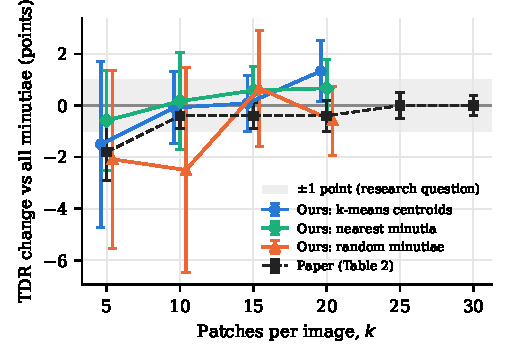
\includegraphics[width=\columnwidth]{tdr_vs_k.pdf}
\caption{TDR at FDR~=~0.2\% against the number of patches. Error bars: s.d.\ over 5 k-means or random
seeds. Dotted lines: all-minutiae baselines.}\label{fig:tdr}
\end{figure}

Table~\ref{tab:main} and Fig.~\ref{fig:tdr} compare like for like where that is possible: same metric,
same operating point, same values of $k$. With all minutiae my model reaches TDR~=~\TDRall\% (bootstrap
s.d.\ \TDRallBootSD) against the paper's 95.7\%. With 10 centroid patches it reaches
\TDRkTen~$\pm$~\TDRkTenSD\%, a change of \DeltaKTen\ points against the paper's $-0.4$. At FDR~=~1\% the two
are \TDRallOne\% and \TDRkTenOne\%.
\todo{2--3 sentences in your own words: does k=10 meet the 1-point criterion? Is the absolute level close
to 95.7\%? At which k does TDR stop changing, and is that the same as the paper's (about 10)?}

\section{Numbers the paper does not report}
\begin{table}[t]
\centering\caption{Patch-selection ablations, TDR (\%) at FDR~=~0.2\%, mean $\pm$ s.d.\ over 5 seeds.
``Unweighted'': plain mean of centroid patch scores. ``Nearest minutia'': same clusters and weights,
patch centred on the minutia closest to each centroid. ``Random'': $k$ random minutiae.}
\label{tab:abl}\resizebox{\columnwidth}{!}{\begin{tabular}{r rrrr}
\toprule
$k$ & centroid (paper) & unweighted & nearest minutia & random \\
\midrule
5 & 33.9 $\pm$ 3.2 & 34.1 $\pm$ 3.5 & 34.8 $\pm$ 1.9 & 33.3 $\pm$ 3.4 \\
10 & 35.3 $\pm$ 1.4 & 36.8 $\pm$ 1.1 & 35.6 $\pm$ 1.9 & 32.9 $\pm$ 4.0 \\
15 & 35.5 $\pm$ 1.1 & 37.3 $\pm$ 1.4 & 36.0 $\pm$ 0.9 & 36.1 $\pm$ 2.3 \\
20 & 36.8 $\pm$ 1.2 & 38.5 $\pm$ 1.5 & 36.1 $\pm$ 1.1 & 34.8 $\pm$ 1.3 \\
\midrule
All & \multicolumn{4}{c}{35.4 $\pm$ 4.1 (bootstrap s.d.)} \\
\bottomrule
\end{tabular}
}
\end{table}

\textbf{Is it the clustering, or just fewer patches?} The paper never compares k-means against simply
classifying $k$ minutiae chosen at random. At $k=10$, random minutiae give \TDRrandTen~$\pm$~\TDRrandTenSD\%
against \TDRkTen~$\pm$~\TDRkTenSD\% for centroids (Table~\ref{tab:abl}).
\todo{interpret: if random is as good, the gain comes from averaging fewer patches, not from where they are.}

\textbf{Does the size weighting matter?} Without weights, 10 centroids give
\TDRunwTen~$\pm$~\TDRunwTenSD\%. \todo{interpret.}

\textbf{A second training seed.} Retraining with a different seed gives TDR~=~\TDRallSeedOne\% for all
minutiae (Table~\ref{tab:seeds}).
\todo{compare the seed-to-seed difference with the k=10 vs all difference. If they are similar in size,
the paper's 0.4-point gap is within training noise.}

\begin{table}[t]
\centering\caption{Two training seeds. ``Fixed thr.'': the all-minutiae threshold reused for $k=10$
instead of recomputing it, as stated in my proposal.}
\label{tab:seeds}\resizebox{\columnwidth}{!}{\begin{tabular}{c rrr}
\toprule
Model seed & All, TDR@0.2 & $k{=}10$, TDR@0.2 & $k{=}10$, fixed thr. TDR / FDR \\
\midrule
0 & 35.4 $\pm$ 4.1 & 35.3 $\pm$ 1.4 & 36.9 / 0.25 \\
1 & 37.9 $\pm$ 7.1 & 34.8 $\pm$ 2.6 & 38.6 / 0.30 \\
\bottomrule
\end{tabular}
}
\end{table}

\textbf{Same threshold for every setting.} The paper recomputes the threshold for each $k$. A deployed
system would keep one. Reusing the all-minutiae threshold at $k=10$ gives TDR~=~\FixedTDRkTen\% at an
actual FDR of \FixedFDRkTen\% (Table~\ref{tab:seeds}). \todo{interpret: does the score distribution shift
when you change the patches?}

\section{What did not reproduce}
\subsection{The speed-up}
\begin{figure}[t]
\centering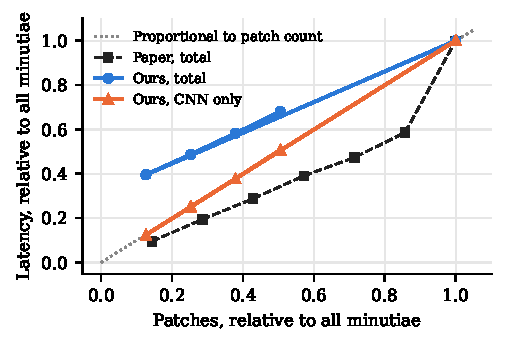
\includegraphics[width=\columnwidth]{relative_latency.pdf}
\caption{Latency against patch count, both relative to all minutiae. The dotted line is latency
proportional to patch count. The paper's points fall below it.}\label{fig:lat}
\end{figure}
\begin{table}[t]
\centering\caption{My per-image latency (ms) by stage: one CPU thread, TFLite with 8-bit weights,
100 test images. Minutiae extraction is the same for every $k$.}
\label{tab:timing}\resizebox{\columnwidth}{!}{\begin{tabular}{r rrrrrr}
\toprule
$k$ & patches & minutiae & select & cut & CNN & total \\
\midrule
All & 39.6 & 72 & 0.0 & 1.8 & 82 & 156 \\
5 & 5.0 & 72 & 2.9 & 0.3 & 11 & 86 \\
10 & 10.0 & 72 & 3.2 & 0.5 & 21 & 97 \\
15 & 15.0 & 72 & 3.9 & 0.7 & 32 & 108 \\
20 & 20.0 & 72 & 4.5 & 0.9 & 42 & 119 \\
\bottomrule
\end{tabular}
}
\end{table}
Cutting the patches from \CallsAll\ to 10 makes the CNN stage \SpeedupCNN$\times$ faster, roughly in
proportion to the patch count, as expected. The whole pipeline, however, goes from \MsAll~ms to
\MsKTen~ms, only \SpeedupTotal$\times$ (Table~\ref{tab:timing}). The reason is minutiae extraction, which
takes \MsMinutiae~ms per image whatever $k$ is: clustering needs the minutiae first, so it can only shrink
the CNN stage. The paper does not say whether its 302~ms includes minutiae extraction. If it does, a
phone extracting minutiae in a small fraction of that time would need a much faster extractor than mine.

\subsection{Table~2 is not internally consistent}
Three things in the paper do not add up, and they bear directly on the claim.
\begin{enumerate}
\item \textbf{Latency per patch.} For $k=5$ to 30, Table~2 implies about 30~ms per patch
(148/5, 302/10, 910/30), which matches the 30~ms per quantised patch quoted in Section~3. At that rate,
all 35 minutiae would take about 1,050~ms, not 1,554~ms. The baseline therefore carries about 500~ms that
the clustered rows do not. Fig.~\ref{fig:lat} shows this: the paper's points fall below the proportional
line, which is impossible if cost only scales with patches. The claimed 5.1$\times$ speed-up
(1,554/302) is larger than the 3.5$\times$ cut in patches (35/10). The paper itself calls it
``approximately 4-fold'' in one place and ``almost 80\%'' in another. I cannot tell whether the baseline
was timed differently, for example unquantised, or includes extra work.
\item \textbf{The baseline TDR.} Section~2.4 reports TDR~=~97.20\% at FDR~=~0.2\% when all materials are
known in training. Table~2's all-minutiae row, also with all materials known, is 95.7\%. The paper does
not reconcile them. The cause could be the $96\times96$ retraining, quantisation or a different split.
\item \textbf{What the s.d.\ measures.} The all-minutiae row has s.d.\ 0.1 although it involves no k-means
at all. That variation must come from something other than k-means initialisation, which suggests the
``5 folds'' are five data splits. If so, the $\pm0.5$ at $k=10$ mixes split noise with initialisation
noise. My s.d.\ over k-means seeds on one split is not the same quantity, so the error bars in
Table~\ref{tab:main} are not strictly like for like.
\end{enumerate}

\subsection{The operating point is fragile}
At FDR~=~0.2\% with 1,000 bona fide images, the threshold is set by the third-highest bona fide score, so
one or two unusual bona fide prints decide the result. My bootstrap s.d.\ for the baseline is
\TDRallBootSD\ points, against the paper's 0.1 over its folds. A gap of 0.4 points (95.7 vs 95.3) is
\todo{smaller / larger} than this sampling error, so the paper's data alone cannot show that $k=10$ and
all minutiae differ, or that they are the same.

\subsection{What I tried}
The model is trained on minutia-centred patches but tested on centroid-centred ones, and a centroid
often falls between minutiae. To check whether this mismatch costs accuracy, I moved each patch to the
minutia nearest its centroid, keeping the same clusters and weights. This gave
\TDRnearTen~$\pm$~\TDRnearTenSD\% at $k=10$ (Table~\ref{tab:abl}).
\todo{interpret. Add anything else you tried, e.g.\ a change you made after a first run and why.}

\subsection{What I still cannot explain}
\todo{Be specific: e.g.\ the remaining gap in absolute TDR level and which of (extractor, training
schedule, split, dataset) you think causes it and why you could not test it; the 500~ms in the paper's
baseline.}

\section{Data ethics}
Fingerprints are biometric data about identifiable people. MSU-FPAD and PBSKD are released for academic
research under a data agreement with Michigan State University.
\todo{State the agreement's terms in your words: who signed, permitted use, redistribution, whether
subjects consented to research use, and whether committing trained weights is allowed.}
I therefore commit no images, patches or minutiae. Minutiae coordinates are themselves a biometric
template, so the minutiae cache stays out of the repository. The illustrative figure uses a synthetic
fingerprint. The repository contains only file names, anonymous per-image scores and trained weights.
Presentation-attack detection is dual-use: the per-material results could also show an attacker which
materials evade the detector.

\section{Conclusion}
\todo{3--4 sentences: what reproduced, what did not, and the one number you would defend first in the
viva.}

\section*{Use of AI tools}
The code and a first draft of this write-up were produced with the help of an AI assistant (Claude). I ran
every experiment, checked the code, and wrote or rewrote the interpretation.
\todo{Adjust to match exactly what you did.}

\begin{thebibliography}{9}
\bibitem{chugh2019} T.~Chugh and A.~K.~Jain, ``Fingerprint presentation attack detection: Generalization
and efficiency,'' in \emph{Proc. ICB}, 2019. arXiv:1812.11574.
\bibitem{chugh2018} T.~Chugh, K.~Cao, and A.~K.~Jain, ``Fingerprint Spoof Buster: Use of minutiae-centered
patches,'' \emph{IEEE Trans. Inf. Forensics Security}, vol.~13, no.~9, pp.~2190--2202, 2018.
\bibitem{howard2017} A.~G.~Howard \emph{et al.}, ``MobileNets: Efficient convolutional neural networks for
mobile vision applications,'' arXiv:1704.04861, 2017.
\end{thebibliography}
\end{document}
